
In this section, we will develop some general intuitions about system integration and then
give precise definitions in {\MMT}. A particular strength of {\MMT} is that we can give
these precise definitions without committing to a particular foundational system and thus
without loss of generality.

The typical integration situation is that we have two systems  for  that
implement a shared specification . For example, these systems can be computer algebra
systems or (semi-)automated theorem provers. Our integration goal is to move problems and
results between  and .



\paragraph{Specifications and Systems}
Let us first assume a single system  implementing , whose properties are
given by logical consequence relations  and . We call
 \emph{sound} if  implies  for every formula 
in the language of . Conversely, we call  \emph{complete} if  implies .

While these requirements seem quite natural at first, they are too strict for practical purposes. It is well-known that soundness fails for many CASs, which compute wrong results by not checking side conditions during simplification. Reasons for incompleteness can be theoretical --- e.g., when  is a first-order prover and  a higher-order specification --- or practical --- e.g., due to resource limitations.

Moreover, soundness also fails in the case of underspecification:  is usually much
stronger than  because it must commit to concrete definitions and implementations
for operations that are loosely specified in . A typical example is the
representation of undefined terms (see~\cite{DBLP:conf/cade/Farmer04} for a survey of
techniques). If  specifies the rational numbers using in particular , and  defines , then  is not sound because
 is not a theorem of . 




We can define the above notions in {\MMT} as follows. A \emph{specification}  is an
{\MMT} theory; its meta-theory (if any) is called the \emph{specification language}. A
system implementing  consists of an {\MMT} theory  and an {\MMT} theory
morphism ; the meta-theory of  (if any) is called the
\emph{implementation language}.  With this definition and using the Curry-Howard
representation of {\MMT}, we can provide a deductive system for the consequence relations used above:
 iff there is a  such that ; and accordingly for
.

In the simplest case, the morphism  is an inclusion, i.e., for every symbol in ,  contains a symbol of the same name. Using an arbitrary morphism  provides more flexibility, for example, the theory of the natural numbers with addition and multiplication implements the specification of monoids in two different ways via two different morphisms.

\begin{example}\label{ex:peano-zf}
  We use a theory for second-order logic as the specification language; it declares
  symbols for , , etc.  is a theory for the natural numbers; it
  declares symbols ,  and  as well as one symbol  for each Peano axiom .

  For the implementation language, we use a theory  for ZF set theory; it has
  meta-theory first-order logic and declares symbols for , , , etc. Then we
  can implement the natural numbers in a theory  declaring, e.g., a symbol
   defined as , a symbol  defined such that , and prove
  one theorem  in  for each Peano axiom.  Note that  yields theorems about
  the natural numbers that cannot be expressed in , for example .
  We obtain a morphism  using ,  etc.
  
  Continuing Ex.~\ref{ex:peano-cic}, we obtain a different implementation  using ,  etc.
\end{example}

To capture practice in formal mathematics, we have to distinguish between the definitional
and the axiomatic method.  The \emph{axiomatic} method fixes a formal system  and then
describes mathematical notions in -theories  using free symbols and axioms.   is
interpreted in models, which may or may not exist. This is common in model theoretical
logics, especially first-order logic, and in algebraic specification.  In {\MMT},  is
represented as a theory with meta-theory  and with only undefined constants. In
Ex.~\ref{ex:peano-zf},  is second-order logic and  is .

The \emph{definitional} method, on the other hand, fixes a formal system  together with
a minimal theory  and then describes mathematical notions using definitional
extensions  of . The properties of the notions defined in  are derived as
theorems. The interpretation of  is uniquely determined given a model of . This is
common in proof theoretical logics, especially LCF-style proof assistants, and in set
theory. In Ex.~\ref{ex:peano-zf},  is first-order logic,  is ZF, and  is
.

\paragraph{Types of Integration}
Let us now consider a specification  and two implementations . To simplify the notation, we will write  and  instead of  and .
We first describe different ways how to integrate  and  intuitively.

\emph{Borrowing} means to use  to prove theorems in the language of . Thus, the input to  is a conjecture  and the output is an expression . In general, since {\MMT} does not prescribe a calculus for proofs, the object  can be a formal proof term, a certificate, proof sketch, or simply a yes/no answer.

\emph{Computation} means to reuse a  computation in . Thus, the input of  is an expression , and the output is a proof  with an expression  such that . To be useful,  should be simpler than  in some way, e.g., maximally simplified or even normalized.

\emph{Querying} means answering a query in  and transferring the results to . This is similar to borrowing in that the input to  is a formula . However, now  may contain free variables, and the output is not only a proof  but also a substitution  for the free variables such that .

In all cases, a translation  must be employed to translate the input from  to
.  Similarly, we need a translation  in the opposite direction to translate the
output  and  and (if available)  from  to .



To define these integration types formally in {\MMT}, we first note that borrowing is a special case of querying if  has no free variables. Similarly, computation is a special case of querying if  has the form  for a variable  that does not occur in . 

\begin{wrapfigure}{r}{2.8cm}
\vspace*{-2.5em}
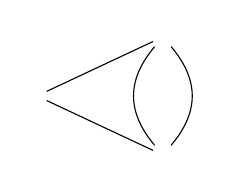
\begin{tikzpicture}[yscale=.5,xscale=.8]
\node (S) at (0,0)
    {};
\node (L1) at (2,1.5)
    {};
\node (L2) at (2,-1.5)
    {};
\draw[-\arrowtip](S) -- node[above,near start] {} (L1);
\draw[-\arrowtip](S) -- node[below,near start] {} (L2);
\draw[-\arrowtip](L1) to[out=-60,in=60] node[right] {} (L2);
\draw[-\arrowtip](L2) to[out=120,in=-120] node[right] {} (L1);
\end{tikzpicture}
\vspace*{-3.5em}
\end{wrapfigure}

To define querying in {\MMT}, we assume a specification, two implementations, and
morphisms  and  as on the right.  and  must satisfy
, , and
. \ednote{CSC: given the first equation, the other two imply each other. Should we make this explicit?} Then we obtain the following \emph{general form of an
  integration problem}: Given an -context  and a query  (where
 denotes the requested proof), find a substitution  and a proof
. Then {\MMT} guarantees that  so that we
obtain  as the solution.
Moreover, only the existence of  is necessary but not  itself --- once a proof  is found in , the existence of  ensures that  is true in , and it is not necessary to
translate  to .
\medskip

We call the above scenario \emph{safe bidirectional communication} between  and  because  and  are theory morphisms and thus guarantee that consequence and truth are preserved in both directions.
This scenario is often implicitly assumed by people coming from the first-order logic community. Indeed, if  and  are automatic or interactive theorem provers for first-order logic, then the logic of the two systems is the same and both  and  are equal to .

If we are only interested in \emph{safe directed communication}, i.e., transferring results from  to , then it is sufficient to require only . Indeed, often  is an inclusion, and the input parameters  and , which are technically -objects, only use symbols from . Thus, they can be moved directly to  and , and  is not needed.


Similarly, the substitution  can often be stated in terms of . In that case,  is only needed to translate the proof . If the proof translation is not feasible,  may be omitted as well.
Then we speak of \emph{unsafe communication} because we do not have a guarantee that the communication of results is correct.
For example, let  and  be two CASs, that may compute wrong results by not
checking side conditions during simplification. Giving a theory morphism  means that
the ``bugs'' of the system  must be ``compatible'' with the ``bugs'' of ,
which is quite unlikely.


The above framework for safe communication via theory morphisms is particularly appropriate for the integration of axiomatic systems. However, if  and  employ different mathematical foundations or different variants of the same foundation, it can be difficult to establish the necessary theory morphisms. In {\MMT}, this means that  and  have different meta-theories so that  and  must include a meta-morphism. Therefore, unsafe communication is often used in practice, and even that can be difficult to implement.

Our framework is less appropriate if  or  are developed using the
definitional method. For example, consider Aczel's encoding of set theory in type
theory~\cite{aczel,werner-zfc}. Here  as in Ex.~\ref{ex:peano-zf}, and
 as in Ex.~\ref{ex:peano-cic}. Azcel's encoding provides the
needed meta-morphism  of . But because  is definitional, we
already have , and we have no freedom to define  such that it maps the concepts of
 to their counterparts in .  Formally, in {\MMT}, this means that the
condition  fails. Instead, we obtain two versions of the natural
numbers in CIC: a native one given by  and the translation of  given by
. Indeed, the latter must satisfy all -theorems including, e.g.,
, which is not even a well-formed formula over . We speak of
\emph{faithful communication} if  can be established even when
 is definitional. This is not possible in {\MMT} without the extension we propose
below.







